% Report template
% Author: Peter Ashcroft, ETH Zurich

\documentclass[a4paper,11pt]{article}
\usepackage{blue}
\usepackage{amsmath}

\usepackage{listings}
\lstnewenvironment{mat}{\lstset{
language=mathematica,
mathescape,
columns=flexible,
%basicstyle={\sffamily\footnotesize},
commentstyle=\color{gray!70},
numbersep=5pt,
breaklines=true,
keywordstyle=\color{color1},
rulecolor=\color{color1},
framerule=0.5pt,
tabsize=2,
backgroundcolor = \color{gray!10},
xleftmargin = 1em,
framexleftmargin = 1em
}}{}


\newcommand{\avg}[1]{\left\langle #1 \right\rangle}

% Personal data
\name{Peter Ashcroft}
\title{St. Petersburg paradox}
\subtitle{}
\address{Institute for Integrative Biology}{ETH Z\"urich}{}%Universit\"atstrasse 16, Z\"urich, 8092}
%\phone{+41~(0)44~633~60~34}
\email{peter.ashcroft@env.ethz.ch}
\homepage{ashcroftp.github.io}
\header{St. Petersburg paradox}

\begin{document}
\maketitlebox

\textbf{What is the probability of running out of money in a game with infinite expected return?}

\section*{Question formulation}
We consider a repeatable game, where the player pays a fixed fee $m$ to enter.
The pot starts at \$1, and doubles each time a head (H) is thrown.
The game stops when the first tail (T) appears, and the player receives the current pot value, i.e.
\begin{equation}
r(\text{T}) = \$1, \quad r(\text{HT}) = \$2, \quad r(\text{HHT}) = \$4, \quad r(\text{HHHT}) = \$8, \quad \dots. \nonumber
\end{equation}

The player begins with a balance of $s$, and can only play the game if $s \ge m$ (i.e. if they have enough money to pay the entry fee).
We want to find $p_m(s)$, which is the probability that the gambler can play the game indefinitely (or that they do not run out of money).

\section*{The paradox}
This game is paradoxical because the expected return, $\avg{r}$, is infinite, so any rational gambler would play, no matter the cost of the entry fee $m$:
\begin{alignat*}{2}
r_n = 2^n &
&&\text{Return after $n$ heads,} \\
p_n = \left(\frac{1}{2}\right)^n\left(1-\frac{1}{2}\right)& \qquad
&& \text{Probability of $n$ heads followed by a tail,} \\
\avg{r} = \left(\sum_{n=0}^\infty p_n r_n\right) - m = \left(\frac{1}{2} \sum_{n=0}^\infty 1\right) - m = \infty & \qquad
&& \text{Expected return.}
\end{alignat*}


\section*{Solution: Markov chain}
The repeated game can be formulated as a Markov chain.
Let $t$ denote the number of games played, and $P_i(t)$ be the probability that we have a balance of $i$ after $t$ games ($i \in \{1,2,\dots\}$, $t \in \{0,1,2,\dots\}$).
Therefore, $P_i(0) = \delta_{i,s}$.
We now want to express $P_i(t+1)$ as a function of $P_i(t)$.
As the states $i<m$ are absorbing (we can't play any more if our balance is less than the entry fee $m$), we write down an equation for the absorbing states and an equation for the remainder:
\begin{subequations}
\begin{alignat}{2}
P_i(t+1) &= \sum_{n \,:\, i-(2^n-m) \ge m} p_n P_{i-(2^n-m)}(t) + P_i(t) \qquad && \text{for}~ 1 \le i < m, \\
P_i(t+1) &= \sum_{n \,:\, i-(2^n-m) \ge m} p_n P_{i-(2^n-m)}(t) \qquad && \text{for}~ m \le i < \infty,
\end{alignat}
\label{eq:MarkovChain}%
\end{subequations}
where the limit on the sum accounts for no transitions out of the absorbing states.

This Markov chain can be forward-integrated, starting form $P_i(0)$, to find the distribution of balances after $t$ games.
The probability that we can continue playing ($i>m$) after this time is then
\begin{equation}
p_m(s) = \lim_{t\to\infty} \left[1- \sum_{i=1}^{m-1} P_i(t)\right].
\end{equation}
To solve the Markov chain computationally we have to impose an artificial upper bound on the size of the state space, as well as on the number of iterations $t$.

The survival probability $p_m(s)$ is shown in Fig.~\ref{fig:StPetersburgOut} for a range of $m$ and $s$ parameters.

\begin{figure}
\centering
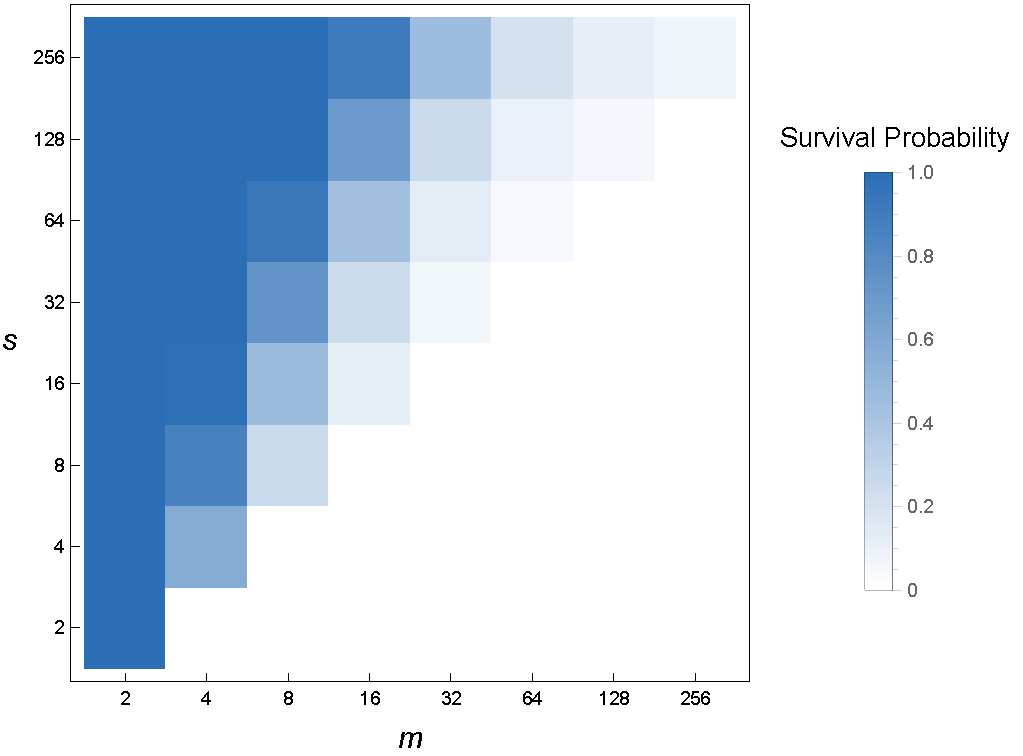
\includegraphics[width=0.5\textwidth]{StPetersburgOut.pdf}
\caption{Survival probability after $2^{10}$ iterations and a state space of size $2^{10}$.}
\label{fig:StPetersburgOut}
\end{figure}

\subsection*{Mathematica code}

\begin{mat}
computeMat[log2nStates_, m_] := Block[{nStates, weights, dim, mat},
  nStates = 2^log2nStates;
  weights = Table[(p^n (1 - p)) /. p -> 0.5, {n, 0, Floor[log2nStates]}];
  dim = {nStates, nStates};
  
  mat = Total[
    Map[
      SparseArray[
        Table[{i, m + i - 2^#} -> weights[[# + 1]], {i, 2^#, Min[nStates - m + 2^#, nStates]}],
        dim] &, 
      Range[0, Floor[log2nStates]]
    ]
  ];
  mat += SparseArray[Table[{i, i} -> 1., {i, 1, m - 1}], dim];
  Return[mat]
]

computeP[log2nStates_, m_, s_, log2nIter_, mat_] := 
 Block[{nStates, nIter, P, Pfinal},
  nStates = 2^log2nStates;
  nIter = 2^log2nIter;
  P = Normal[SparseArray[s -> 1., nStates]];
  Pfinal = Nest[Dot[mat, #] &, P, nIter];
  Return[1. - Sum[Pfinal[[i]], {i, 1, m - 1}]]
]

(*Construct the transition matrix for cost m and state-space size nStates*)
m = 2;
nStates = 2^10;
mat = computeMat[Log2[nStates], m];

s = 2;
nIter = 1000;
survivalProb = computeP[Log2[nStates], m, s, Ceiling[Log2[nIter]], mat]
\end{mat}


\section*{Solution: Linear system}
An alternative approach to this problem is to consider a linear system for the variables $p_m(s)$ themselves.
I.e.
\begin{equation}
p_m(s) = \sum_{n=0}^\infty p_n p_m(s + 2^n-m),
\label{eq:LInearSystem}
\end{equation}
with $p_m(s) = 0$ for $s<m$.
The solution Eq.~\eqref{eq:LInearSystem} is directly related to the stationary solution of Eqs.~\eqref{eq:MarkovChain}.

Computationally, as above, we have to put an upper bound on the state space

\end{document}
